\section{Leveraged ETFs and volatility drag}

\begin{tcolorbox}[width=\linewidth, sharp corners=all, colback=white!95!black]
How would an asset manager build and manage a leveraged ETF? How to cope with volatility drag?
\end{tcolorbox}

Let's say we want to offer a "$2\times$ AAPL" product to our clients. This exchange-traded product should replicate the daily performance of two times the one of the underlying common Apple stock.

\paragraph*{Product design:} Two instruments can be used on top of the udnerlying to deliver a leveraged performance: total return swaps and futures. Following \cite{cheng2009dynamics}, let $S_t$ be the price of one Apple share at time $t$, and $r_i$ be the return of the underlying between $t_{i-1}$ and $t_i$: $r_i = \dfrac{S_{t_{i}}}{S_{t_{i-1}}} - 1$. $r_{i\colon j}$ will denote the return between times $t_i$ and $t_j$. We will denote $x$ the leveraged multiple, which usually takes values in $\{-2, -1, 2, 3\}$.\newline There is a path-dependency in the delivered returns, as the compounded move has no reason to be the same as the multipled return: \[\prod_{i=1}^N (1+xr_i) \neq (1+xr_{0\colon N}).\]

Let's consider the ETP has a NAV of $A_n$ at time $t_n$. The notional of the total return swaps required is $L_n = x A_n$. With a daily rebalancing, at the end of the day the TRS exposure is $x A_n (1+r_{n+1})$ while the fund's NAV grew to $x A_n (1+xr_{n+1})$. To account for this disparity, the exposure to the TRS has to be adjsuted by $\Delta_n = A_n (x^2-x) r_{n+1}$.

\paragraph*{Volatility drag} is the difference between summed and compounded returns: it is harder to recover from a much lower starting point. Indeed, while we need a $20\%$ drop to go from $\$100$ to $\$80$, we need $25\%$ to make it back to $\$100$, and $-20\%+25\% \neq 0$.\newline This is referred to as vol drag, vol tax, or even variance drain.

If we consider a series of fair coin flips where, starting at $\$100$ you bet one percent of your bankroll, double your bet on heads and lose it on tails, with $v_n=100\times 0.99^{n} \times 1.01^n$, you'd have $\forall n \in \mathbb{N}^{*} v_n < 100$ and $\lim_{n \to +\infty} v_n = 0$.

\begin{figure}[H]
    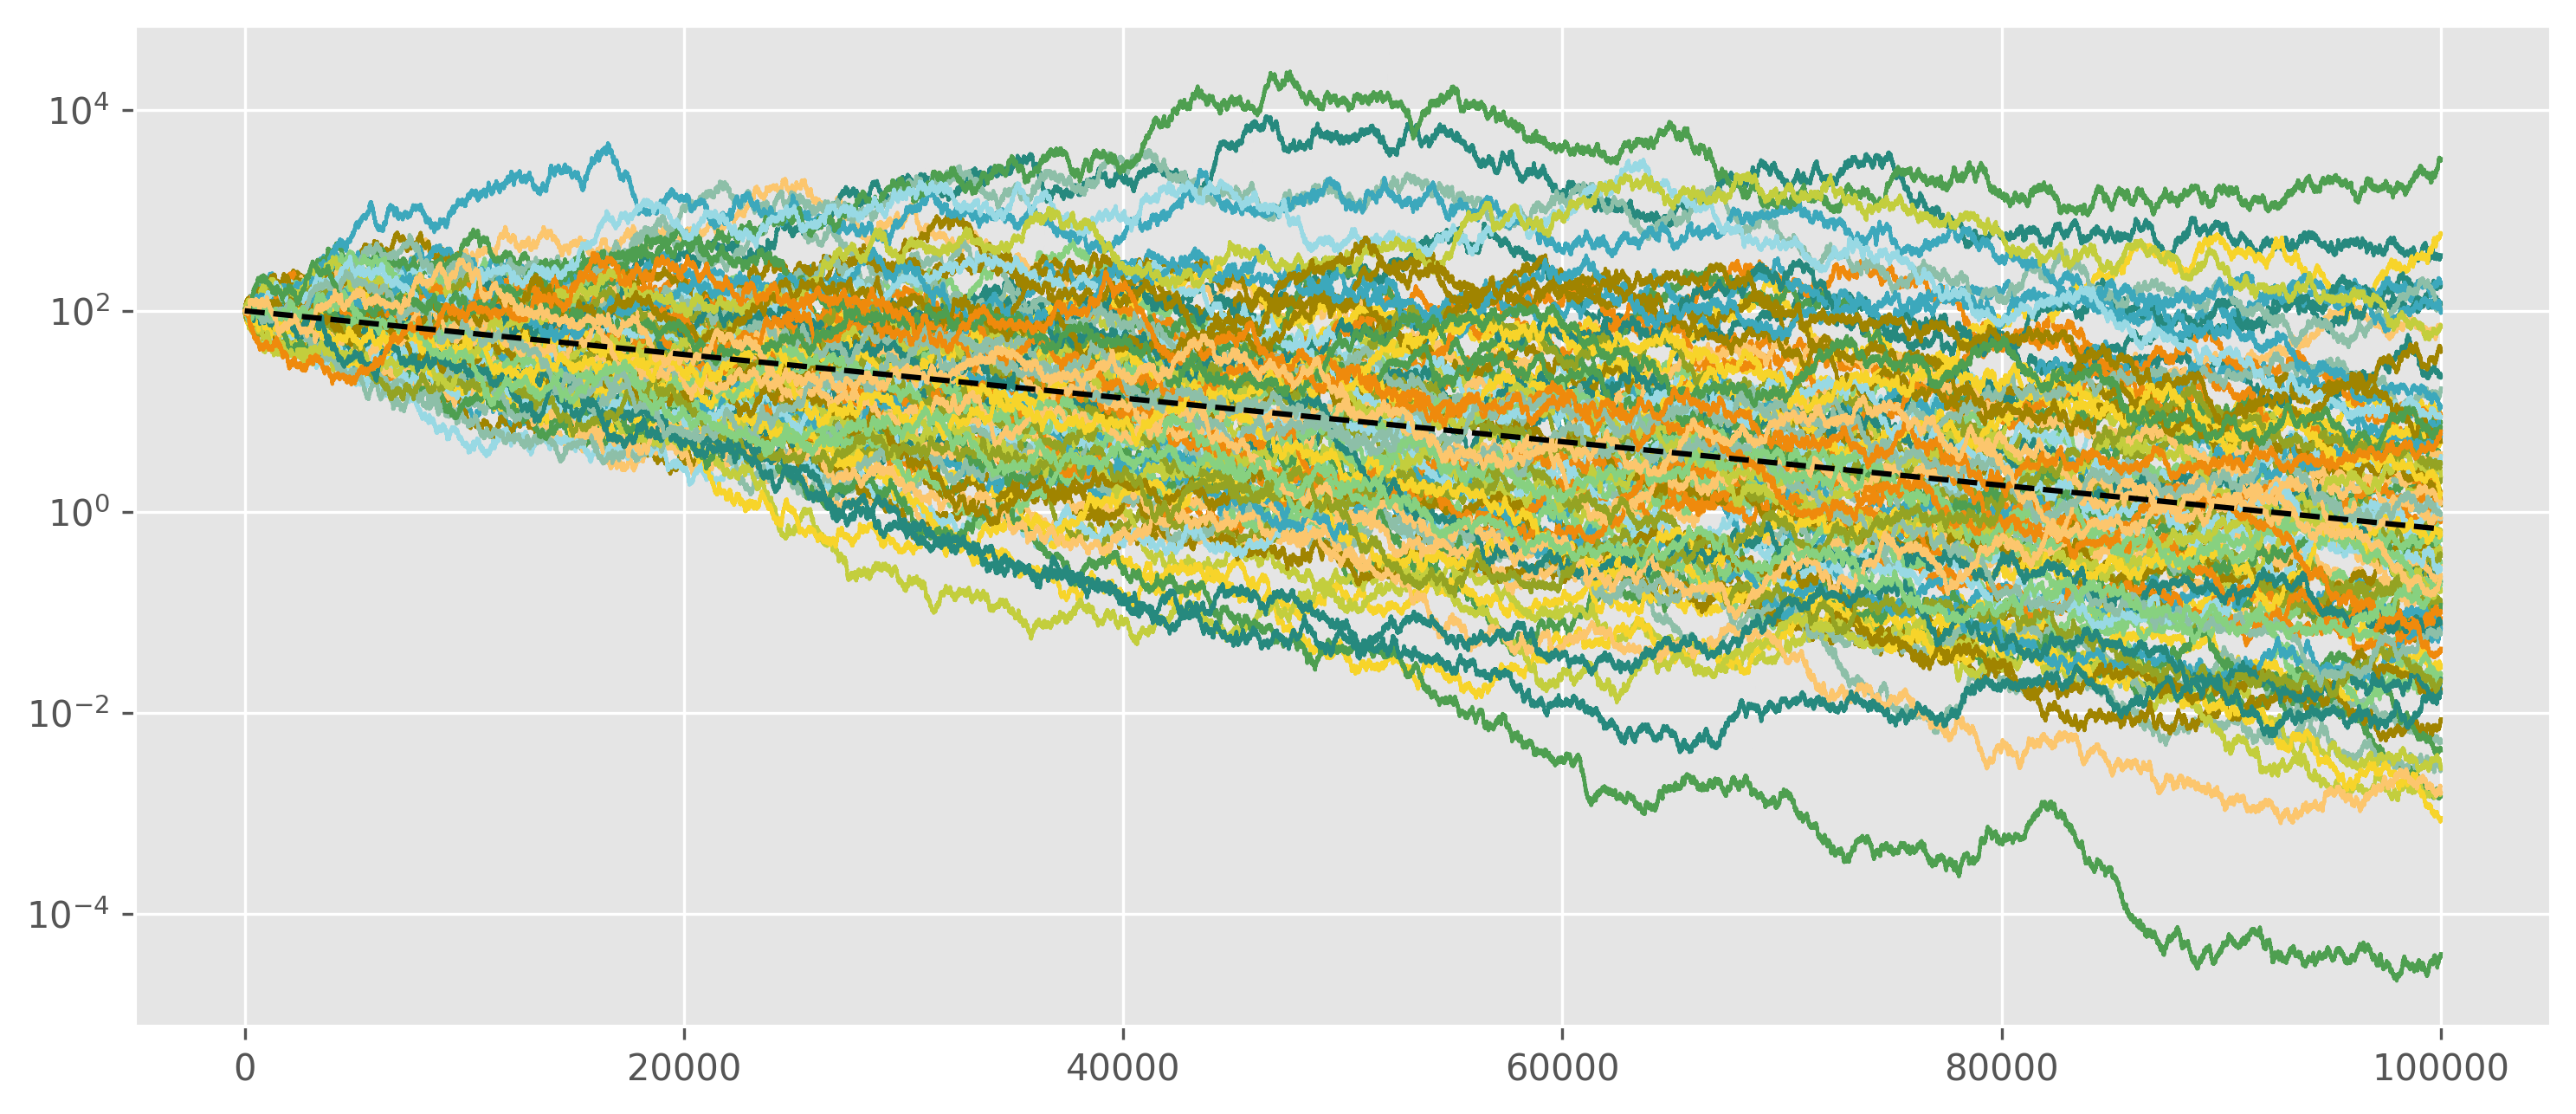
\includegraphics[width=0.85\textwidth]{include/img/coin_flip_drag.png}
    \centering
    \caption{Wealth after $n$ coin flips, with the drag trend. See \href{https://github.com/vtisserand/quant_itws/tree/main/code/snippet/coin_flip_drag.py}{code snippet}.}
    \label{fig:coin_flip_drag}
\end{figure}

Are all leveraged ETFs doomed to ruin though? No, but they appear not suited for long term investors as only a positively skewed return distribution could compensate the effect of the drag.

We can quantity the difference between arithmetic and geometric returns: $r_g \approx r_a - \sigma^2/2$. This applies to all assets, however leveraged products can only amplify this phenomenon and the $2\times$ AAPL product would come with quadruple the volatility drag of owning shares spot, with manager fees.